\documentclass{beamer}

\usepackage[frenchb]{babel}
\usepackage[T1]{fontenc}
\usepackage[utf8]{inputenc}
\usepackage{graphicx}

\usetheme{Warsaw}

\title{Algorithmique Répartie}
\author{Jeremy Krebs - Guillaume Soulié}
\institute{Université Paris Saclay}
\date{\today}

\begin{document}

\begin{frame}
\titlepage
\end{frame}

% --------- Sommaire ---------
\begin{frame}
  \tableofcontents
\end{frame}      
% ----------------------------



\section{Introduction}
\subsection{State of the Art}
\subsubsection{Motivations}
\begin{frame}
\end{frame}
\subsubsection{Related work}
\begin{frame}
\end{frame}
\subsection{Hypotheses}
\begin{frame}
	There are a few hypotheses on the robots:
	\begin{itemize}
		\item<2-> Robots are identical. No distinction, same algorithm,
		\item<3-> Robots are oblivious. They have no memory of their moves,
		\item<4-> Robots cannot communicated directly.
	\end{itemize}
	
	\uncover<5->{However they can observe the positions of the other robots, and it is one of those two cases:}
	\begin{itemize}
		\item<6-> Global-Strong Multiplicity Detection
		\item<7-> Local-Strong and Global-Weak Multiplicity Detection
	\end{itemize}
\end{frame}
\begin{frame}
	The scheduler can be of two types:
	\begin{itemize}
		\item<2->[SSYNC] Semi-Synchronous - For each round, a set of robots are activated/executed at the same time.
		\item<3->[ASYNC] Asynchronous - The robots are activated/executed asynchronously
	\end{itemize}
\end{frame}

\subsection{Problems}
\begin{frame}
	\uncover<1->{
	\textbf{Gathering Problem:}
	The goal of the gathering problem is to group all the robots on the same node.}
	
	\uncover<2->{
	\textbf{Orientation Problem:}
	The goal of the set formation problem is to make the robots gather in a configuration such that:} 
	
	\begin{itemize}
		\item<3-> There is exactly one tower node
		\item<4-> There is a 1-robot block of size l
	\end{itemize}

	\uncover<5->{
	\begin{figure}[h]
   		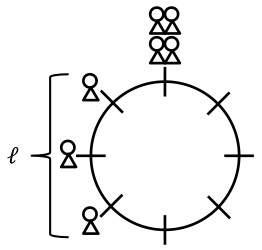
\includegraphics[width=0.3\textwidth]{images/orientation_problem.png}
	\end{figure}}
	
	\uncover<6->{
	\textbf{Set formation problem:}
	The goal of the set formation problem is to gather the robots in a specific predefined configuration.}
\end{frame}

\section{Weaker models}


\section{Gathering Problem}
\begin{frame}
\end{frame}
\section{Orientation Problem}
\begin{frame}
\end{frame}
\section{Set Formation Problem}
\begin{frame}
\end{frame}

\end{document}